
In this section we introduce how the index and data are allocated
on the broadcast channel to form the broadcast program. We
introduce a Tree-based Distributed Index (TDI), our index
allocation technique, which is based on the distributed index
allocation proposed in~\cite{journals/tkde/ImielinskiVB97}. The
benefits of a distributed index over other allocation methods will
be discussed in Section~\ref{sec:wireless_bcast_index}.

We utilize an R-tree~\cite{conf/sigmod/Guttman84} to index our
multi-dimensional data records. We assume that each node of an
R-tree consists of $b$ number of entries, $\{E_1, E_2, ... E_b\}$,
where $b$ is the branching factor, or the number of children at
each internal node, of the index tree, as illustrated by
Figure~\ref{fig:index_node}. Each entry contains a pointer to a
child index node (if the node is not a leaf node), or a pointer to
a set of data records (if the node is a leaf node). The pointer
contains the time when the child item will appear on the broadcast
channel. An advantage of utilizing the R-tree is that the indexed
broadcast data can be employed to support other spatial query
types, such as range~\cite{conf/pods/PagelSTW93} and $k$NN
queries~\cite{journals/tods/HjaltasonS99}.

\subsection{Broadcast Structure}

A broadcast program cycle is a linear representation of the index
tree and data and consists of \emph{index segments} and \emph{data
segments}. Index segments contain temporal pointers to either
another index segment or a data segment. Data segments contain
actual data records. Index and data segments are interleaved to
form a broadcast program. Each index segment is further divided
into smaller units called buckets. Buckets are logical independent
units that represent a portion of the tree index. The purpose for
buckets is that a client does not have to download an entire index
segment if it only needs a bucket.

In addition to a list of temporal pointers, each index bucket also
contains a pointer to the next index segment and a pointer to the
beginning of next broadcast cycle. The purpose of these pointers
is to direct the client to the next index segment in the case that
the client tunes in at the index bucket but is not interested in
the data pointed by the index.

To save bandwidth, data segments do not contain any index
information other than data records. The broadcast program
structure is illustrated in Figure~\ref{fig:index_packet}.

\begin{figure}[!h]
\begin{center}
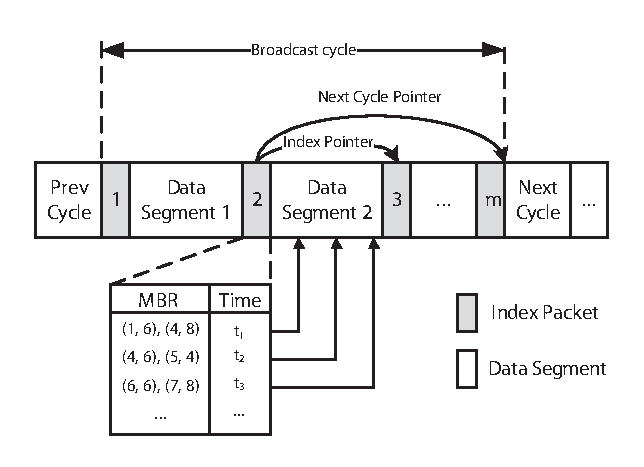
\includegraphics[width=4in]{Figures/index_packet.eps}
\vspace*{-5pt} \caption{Broadcast program cycle format with index
segments and data segments.} \vspace*{-10pt}
\label{fig:index_packet}
\end{center}
\end{figure}

\subsection{TDI Allocation}

After indexing the data set with an R-tree, the next step is to
publish both data and index onto the linear broadcast channel. TDI
allocates space for index and data by performing a depth-first
traversal of the index tree as illustrated in
Figure~\ref{fig:index_struct}. In this process, the root index
node $A$ is first included in the cycle because it is first
traversed. Index node $B_1$ is then included in the program
followed by $C_1$, then the data items $D_1$ and $D_2$. We utilize
depth-first traversal of the index tree instead of breadth-first
traversal in our design because breadth-first traversal cannot
distribute the appropriate portion of index that exactly indexes
the data segment which follows it.

%When an index is replicated, only the MBRs that have not been
%broadcast are published; therefore the replication is not a
%complete replication of the index.

TDI replicates the top $L_r$ levels of the index tree $b$ times,
where the root node is considered level 0. Therefore, the
replication is not an entire path replication of the index. The
replication helps the clients get a broader picture of upcoming
broadcast items. Given $n_i$ to be the current index node to be
broadcast, if the level of $n_i$ is $L_r$ or less, then the parent
of $n_i$ is replicated. Otherwise the parent is not replicated. An
example is shown in Figure~\ref{fig:index_struct}; the root and
the second level index nodes are replicated. Of course, the best
view of upcoming data records would be to replicate the entire
index, but this would be a complete replication, which we try to
avoid to decrease broadcast cycle length.

\begin{figure}[!h]
\begin{center}
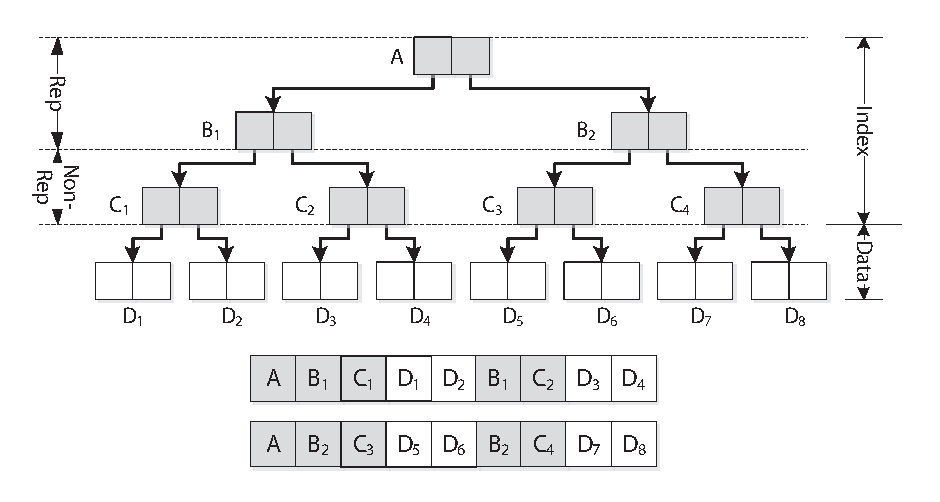
\includegraphics[width=5in]{Figures/bcast_struct.eps}
\caption{Index Structure.} \vspace*{-10pt}
\label{fig:index_struct}
\end{center}
\end{figure}

%and $\varepsilon$ be the space required for an index node entry

\subsection{Analysis}

This section presents the derivation of the two performance
evaluation metrics of the tree-based distributed index, which we
defined in Subsection~\ref{sec:wireless_broadcast}.

\subsubsection{Index Percentage}

Index percentage measures the space overhead of the index
structure. It is defined as the ratio between the space allocated
to the index on the broadcast cycle to the length of the entire
broadcast cycle.

Let $L_r$ be the levels of replication (for example, $L_r$ for the
TDI in Figure~\ref{fig:index_struct} is 2) and $\eta$ be the space
required for an index node. The number of nodes replicated in the
cycle is $(\displaystyle\sum\limits_{i=0}^{L_r-1} b^i)$. In TDI,
each replicated index node appears $b$ times in one cycle.
Consequently, the total space taken by the index is the space for
all index nodes plus the additional space for replication. It is
given by:

\begin{equation}
\delta = \eta\{(\displaystyle\sum\limits_{i=1}^{h-1} b^i + 1) +
(\displaystyle\sum\limits_{i=0}^{L_r-1} b^i)(b - 1)\}
\end{equation}

The length of the broadcast cycle $\omega$ is the space of the
index plus the space of the data ($\delta+\theta$). Therefore, the
index percentage is defined as:

\begin{equation}
\rho = \frac{\delta}{\omega}
\end{equation}

\subsubsection{Initial Index Probe}

The tree-based distributed index divides the entire data set into
smaller data segments and reduces the initial probe of the first
index segment. The length of each data segment, denoted by $\ell$,
is determined by the number of index segments distributed among
the broadcast cycle. As one can see in
Figure~\ref{fig:index_struct}, there are four leaf nodes in the
index and the data is divided into four segments. Therefore, the
number of data segments is $b^{L_r}$ and the size per data segment
is:

\begin{equation}
\ell = \frac{\theta}{b^{L_r}}
\end{equation}

The initial index probe is half of the length of an index segment
plus a data segment:

\begin{equation}
\lambda = \frac{1}{2}(\frac{\delta}{b^{L_r}}+\ell)
\end{equation}

%This is a significant time reduction compare with one-time index
%probe.

%\subsection{Motivation for DFDI}
%Consider that we have an R-tree to index our multi-dimensional data, we
%need to consider the broadcast structure and format so that the index
%and data packets can be broadcasted on the same channel. Tree index
%structures are of particular interest since trees are non-linear whereas
%broadcast program is strictly linear.

%Given two sibling index nodes $A$ and
%$B$ and their parent index node $P$, the following rules determine if
%an index node is replicated in the broadcast program:
%
%\begin{enumerate}
%\item If $A$ is the current index, and $P$ is part of the replicated
%        portion of the index, then $A.ind\_ptr$ points to an index packet
%        and segment that contains both $P$ and $B$.
%\item If $A$ is the current index, and $P$ is \emph{not} part of the
%        replicated portion of the index, then $A.ind\_ptr$ points to
%        an index packet (or segment) that contains only $B$.
%\end{enumerate}

%The broadcast algorithm based on our tree-based distributed index
%is formalized in Algorithm~\ref{alg:TDI}.
%
%\begin{algorithm}
%\algsetup{linenosize=\small,linenodelimiter=. }
%\caption{TDI($Node$, $Level$, $L_r$)} \label{alg:TDI}
%\begin{algorithmic}[1]
%
%\STATE PushToChannel($Node$) \COMMENT{Assume temporal ptrs are
%known} \IF{$Node$ is Leaf}
%    \FORALL{DataSegment in $Node$}
%        \STATE PushToChannel(DataSegment)
%    \ENDFOR
%\ELSE
%    \FORALL{ChildNode in $Node$}
%        \STATE TDI(ChildNode, $Level$++)
%        \IF{$L_r$ $\leq$ $L$ AND NOT Last ChildNode}
%            \STATE PushToChannel($Node$)
%            \COMMENT{Replication}
%        \ENDIF
%    \ENDFOR
%\ENDIF
%\end{algorithmic}
%\end{algorithm}
